\documentclass[a4paper, 12pt]{book}
\usepackage{geometry}
\geometry{a4paper,scale=0.8}
\usepackage[T1]{fontenc}

\usepackage{graphicx}
\usepackage{pythonhighlight}
\graphicspath{ {./images/} }
\usepackage{amsmath}
\usepackage{xcolor} 
\definecolor{deepgreen}{HTML}{006400}
\usepackage{tcolorbox}
\usepackage{listings}
\lstset{
	language=Matlab, % 设定语言为MATLAB
	basicstyle=\ttfamily\footnotesize, % 基本字体样式
	keywordstyle=\color{blue}, % 关键字颜色
	stringstyle=\color{red}, % 字符串颜色
	commentstyle=\color{green!70!black}, % 注释颜色
	backgroundcolor=\color{gray!10}, % 代码背景颜色
	frame=single, % 给代码块加框
	breaklines=true, % 自动换行
	captionpos=b, % 标题位置
	keepspaces=true % 保持空格
}


\begin{document}
	\title{Machine Learning}
	\author{CS229}
	\maketitle
	
	\tableofcontents
	
	\chapter{Linear Regression}
	
	\section{Linear regression with one variable}
	\textbf{target}: predict profits \\
	\textbf{data}: ex1data1.txt - population(just one feature) | profit
	
		\subsection{Plotting the data}
	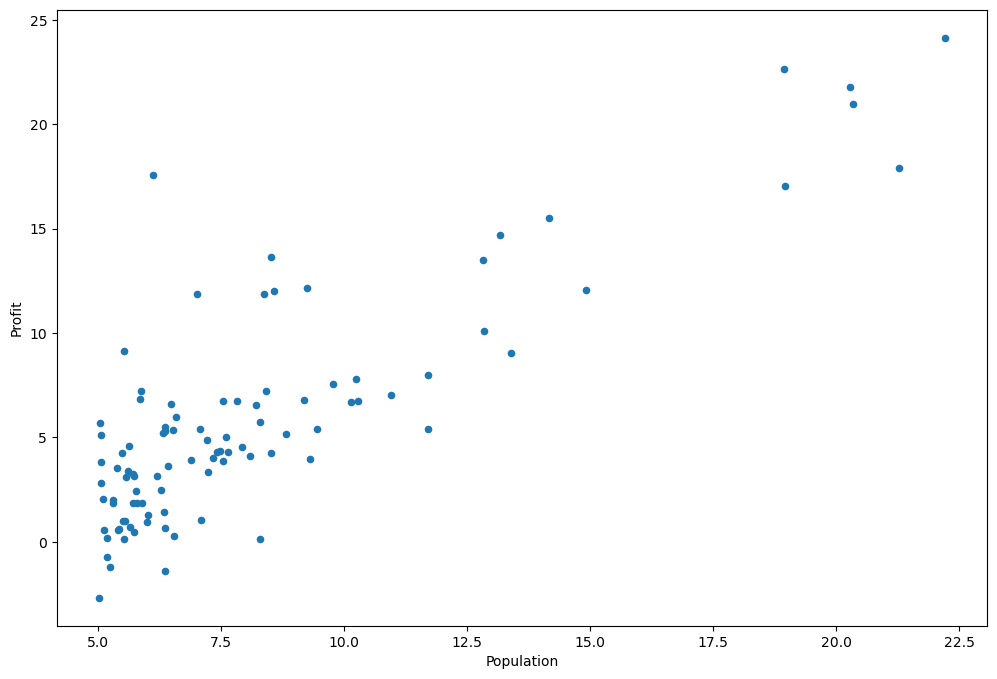
\includegraphics[width=15cm,keepaspectratio]{data}
	
		\subsection{Gradient Descent}
	\textbf{target:} fit $\theta$ to dataset ($\theta$: to minimize cost $J(\theta)$) \\
	\textbf{variable:} x - feature
			\subsubsection{Update Equations}
	\textbf{cost function:} $$J(\theta)=\frac{1}{2m}\sum_{i=1}^{m}(h_\theta(x^{(i)})-y^{(i)})^2$$
	\textbf{hypothesis:}
	$$h_\theta(x)=\theta^Tx=\theta_0+\theta_1x_1(+...+\theta_nx_n)$$
	
				\begin{python}
		
	def computeCost(X, y, theta):
		inner = np.power(((X * theta.T) - y), 2)
		return np.sum(inner) / (2 * len(X))
				\end{python}

	\textbf{in batch gradient descent:}
	$$\theta_j:=\theta_j=\alpha\frac{1}{m}\sum_{i=1}^{m}(h_\theta(x^{(i)})-y^{(i)})x^{(i)}_j$$
	
				\begin{python}

	def gradientDescent(X, y, theta, alpha, iters):
		temp = np.matrix(np.zeros(theta.shape))
		parameters = int(theta.ravel().shape[1])
		cost = np.zeros(iters)
		
		for i in range(iters):
			error = (X * theta.T) - y
		
			for j in range(parameters):
				term = np.multiply(error, X[:,j])
				temp[0,j] = theta[0,j] - ((alpha / len(X)) * np.sum(term))
			
			theta = temp
			cost[i] = computeCost(X, y, theta)
		
		return theta, cost
				\end{python}

		\subsection{Computing the cost $J(\theta)$}
			\subsubsection{Implementation}

				\begin{python}
		
	alpha = 0.01
	iters = 1000
	Theta, cost = gradientDescent(X, y, theta, alpha, iters)
	computeCost(X, y, Theta)
				\end{python}
		\subsection{Visualizing regression}
	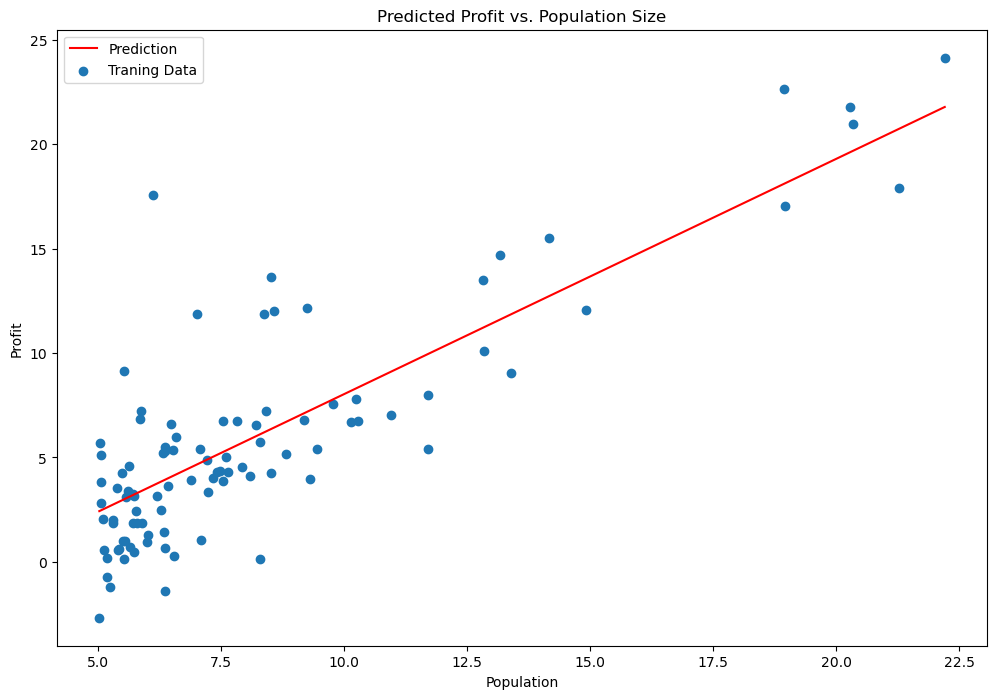
\includegraphics[width=15cm,keepaspectratio]{regression}

		\subsection{Visualizing $J(\theta)$}
		\ \ \ \ \ \ \ 
	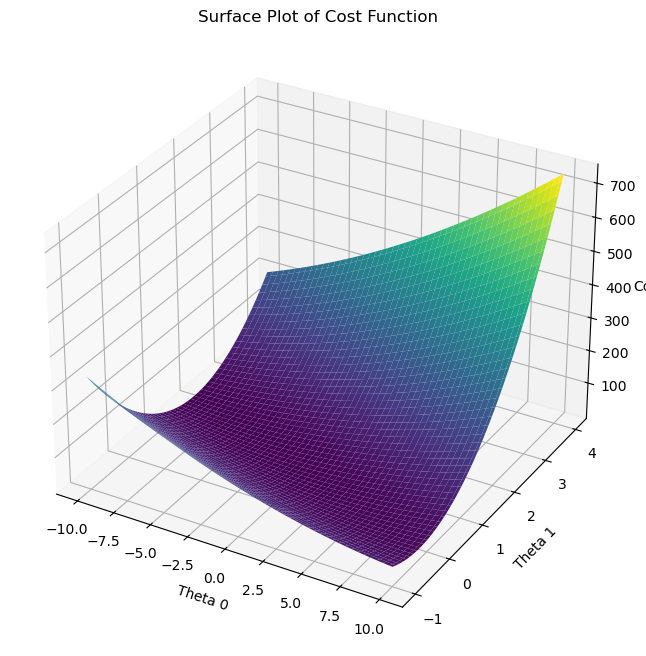
\includegraphics[height=6cm,keepaspectratio]{surface} \ \ \ \ \ \ \ \ \ \ \ \ \ \ \ \ \
	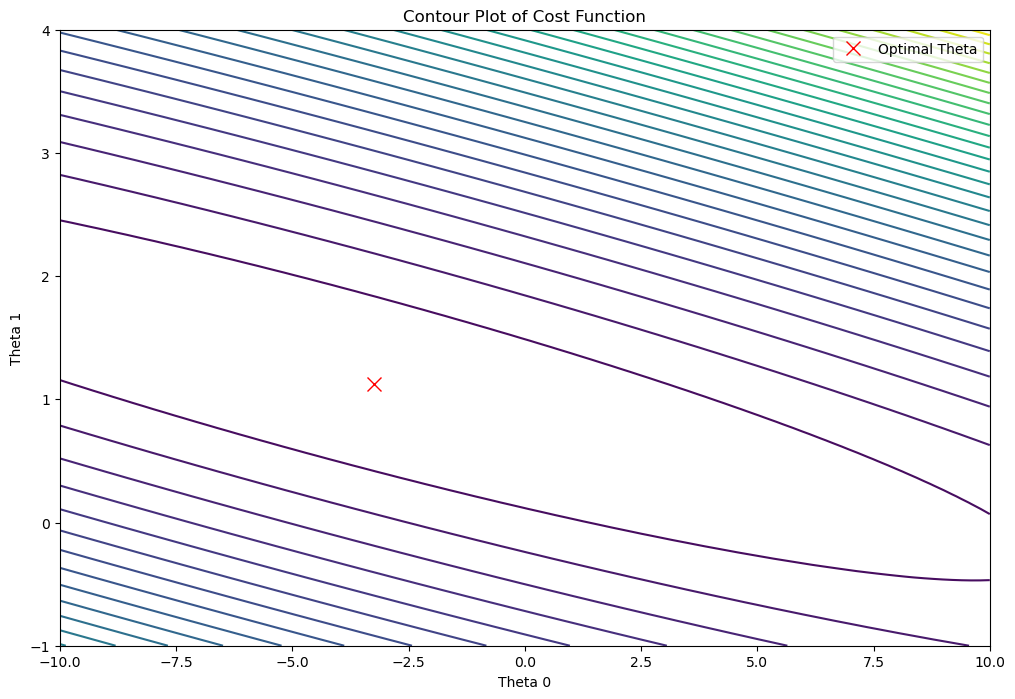
\includegraphics[height=6cm,keepaspectratio]{contour}
	
	\section{Linear regression with multiple variables}
	\textbf{multiple variables: } \\
	\textbf{target: } predict the prices of  houses
		\subsection{Feature Normalization} 
		\ \ \ When features \underline{differ by orders of magnitude}, first performing feature scaling can make gradient descent converge much more quickly. \\ \\
	\textbf{formula: } \\
	$$z=\frac{x-\mu}{\sigma}$$ \\
	{\footnotesize
	mean = $\mu$ \\
	standard deviation = $\sigma$ 
	} \\ \\ \textbf{results: } \\ \\
	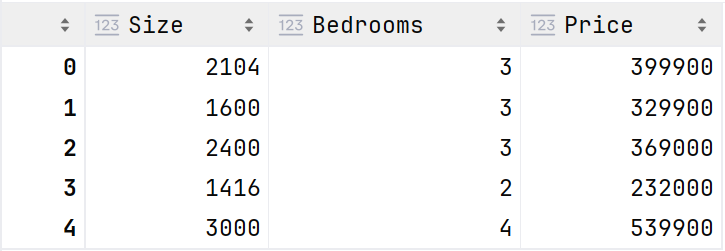
\includegraphics[width=8cm,keepaspectratio]{head} 
	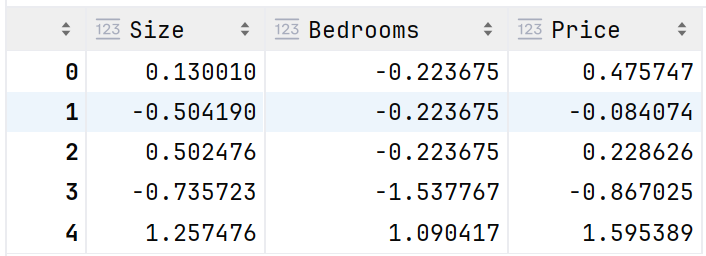
\includegraphics[width=8cm,keepaspectratio]{normalized} \\ \\
	alternative: max-min
		\subsection{Gradient Descent}
			\subsubsection{Update Equations}
	\textbf{cost function:} $$J(\theta)=\frac{1}{2m}(X\theta-\vec{y})^T(X\theta-\vec{y})$$
	where \\
	\[
	X=
	\begin{bmatrix}
		- & (x^{(1)})^T & - \\
		- & (x^{(2)})^T & - \\
		  &   \vdots  &   \\
		- & (x^{(m)})^T & - 
	\end{bmatrix} \ \ \ \ \ \ \
	\vec{y}=
	\begin{bmatrix}
		y^{(1)} \\ y^{(2)} \\ \vdots \\ y^{(m)}
	\end{bmatrix}
	\]
			\subsubsection{Selecting learning rates}
	try out different learning rates \\
	\textcolor{red}{find a learning rate that converges quickly} - less than 50 iterations
	\begin{center}
	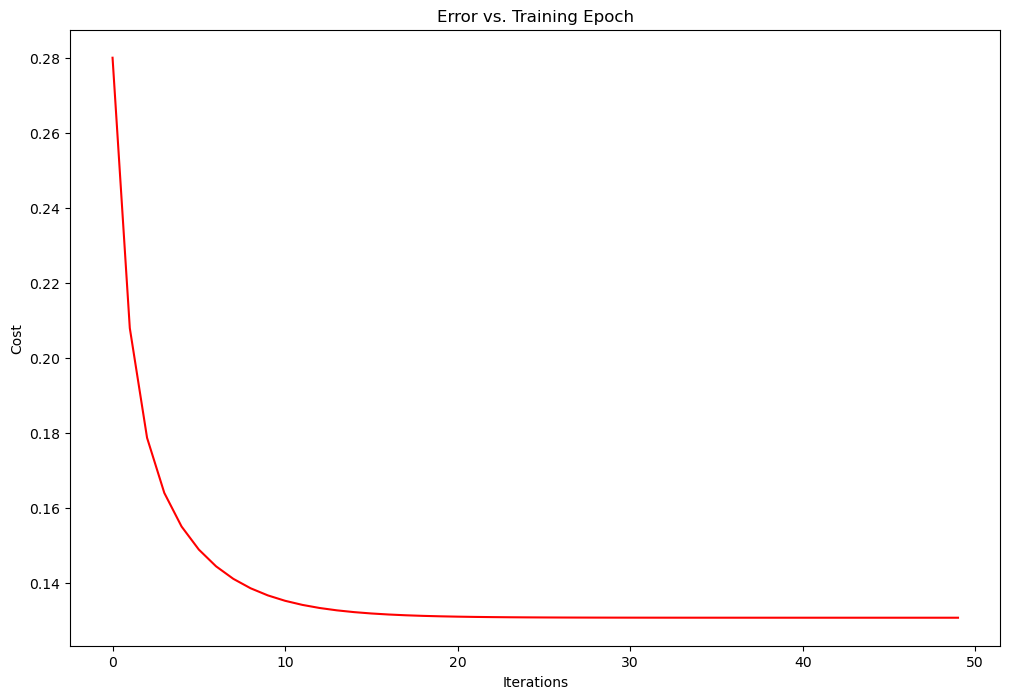
\includegraphics[width=10cm]{epoch2} 
	\end{center}
		\subsection{Normal Equations}
	\textbf{step1.find $\theta$} \\
	closed form solution to linear regression: 
	$$\theta=(X^TX)^{-1}X^T\vec{y}$$
	{\footnotesize
		- does not require any feature scaling \\
		- will get an exact solution in one calculation \\
		- no "loop until convergence" like in gradient descent
	} \\ \\
	\textbf{step2.predict} \\
	make a price prediction for a 1650-square-foot house with 3 bedrooms with $\theta$
	
	
	
	\chapter{Logistic Regression}
	
	\section{Logistic Regression}
	
	\colorbox{deepgreen}{\textcolor{white}{\textbf{\texttt{only able to find a linear decision boundary}}}}\\
	
	\noindent \textbf{target: }predict whether a student gets permitted into a university \\
	\indent \indent - by building a classfication model \\
	\textbf{data: }historical data from previous applicants \\ \indent \indent (scores on two exams and the admissions decision) \\ \indent \indent - as a training set for logistic regression
		\subsection{Visualizing the data}
	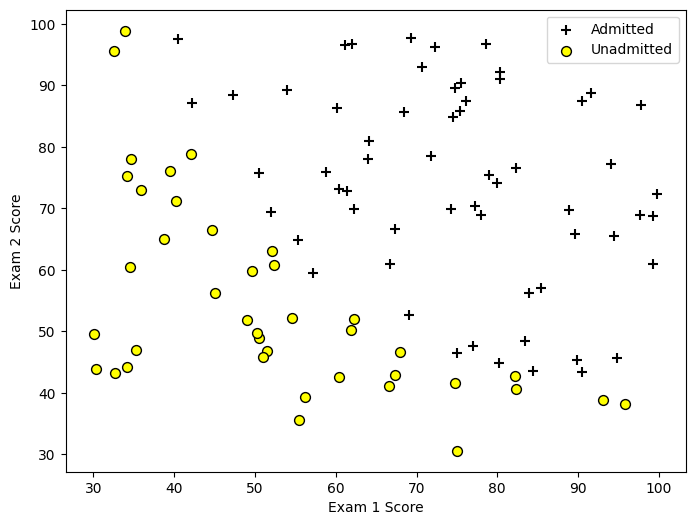
\includegraphics[width=12cm]{data2} 
		\subsection{Implementation}
			\subsubsection{Sigmoid Function}
	\textbf{logistic regression hypothesis: }
	\[h_\theta(x)=g(\theta^Tx)\]
	where $g$ is the \textbf{sigmoid function: }
	\[g(z)=\frac{1}{1+e^{-z}}\]
			\subsubsection{Cost function and gradient}
	\textbf{cost function} in logistic regression:
	\[
		J(\theta)=\frac{1}{m}\sum_{i=1}^{m}[-y^{(i)}\log(h_\theta(x^{(i)}))-(1-y^{(i)})\log(1-h_\theta(x^{(i)}))]
	\]
	\textbf{gradient of the cost: } (a vector of same length as $\theta$)\\
	the $j^{th}$ element (for j = 0, 1,...,n):
	\[
		\frac{\partial{J(\theta)} }{\partial {\theta_j}}
		=
		\frac{1}{m}  \sum_{i=1}^{m}  (h_\theta(x^{(i)}) - y^{(i)} ) x_j^{(i)}
	\]
	{\bfseries\colorbox{pink}{Note:}} while this gradient looks identical to the linear regression gradient, the formula is actually different because linear and logistic regression
	 have different definitions of \(h_\theta(x)\)
	 		\subsubsection{Learning parameters using fminunc (scipy.optimize.fmin\_tnc in Python instead) }
	  \begin{python}
	  	
	import scipy.optimize as opt
	result = opt.fmin_tnc(func=cost, x0=theta, fprime=gradient, args=(X, y))	
	theta_min = np.matrix(result[0])
	 \end{python}
 			\subsection{Visualing regression}
 	\begin{python}
 		
	x = np.linspace(data['Exam 1'].min(),data['Exam 1'].max(),100)
	decision_boundary = -(theta_min[0,1]*x+theta_min[0,0]) / theta_min[0,2]
 	\end{python}
	 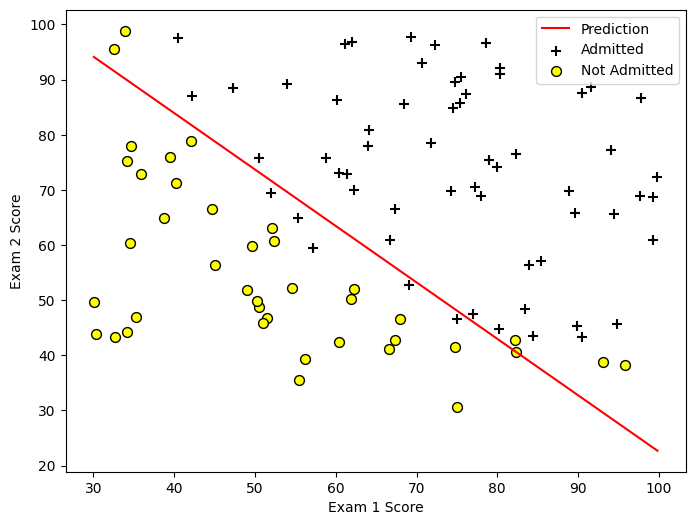
\includegraphics[width=15cm]{boundary}
	 		\subsubsection{Evaluating logistic regression} 
	 After learning the parameters, we can use the model to predic whether a particular student will be admitted. For a student with an Exam 1 score of 45 and an Exam 2 score of 85, you should expect to see an admission probability of 0.776.
	 
	 \begin{python}
	 	
	def predict(theta, X):
		probability = sigmoid(X * theta.T)
		# return [1 if x >= 0.5 else 0 for x in probability]
	 	return probability
	 	
	predict(theta_min, [1,45,85])[0,0]
	 \end{python}
	 \section{Regularized logistic regression}
	 	\subsection{Visualizing the data}
	 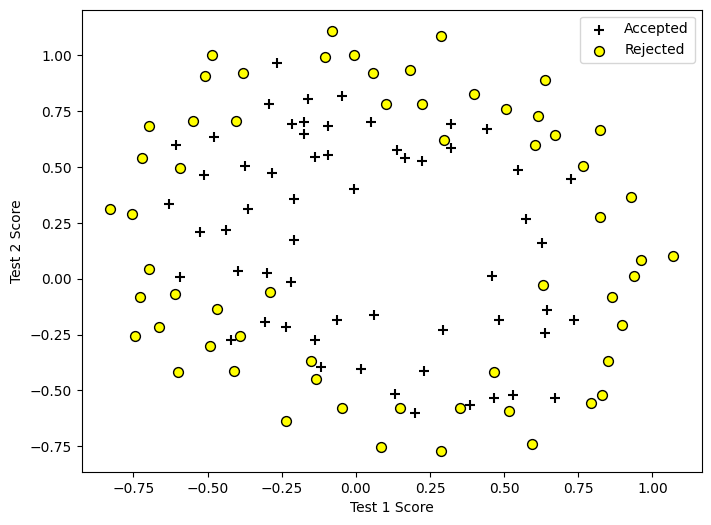
\includegraphics[width=12cm]{data22} 
	 	\subsection{Feature mapping}
	 One way to fit the data better is to create more feature form each data point.——map the features into all polynomial terms of \(x_1\) and \(x_2\) up to the sixth power.
	 \[\
	 mapFeature(x) = 
	\begin{bmatrix}
		1 \\ x_1 \\ x_2 \\ x_1^2 \\ x_1x_2 \\ x_2^2 \\ x_1^3 \\ \vdots \\ x_1x_2^5 \\ x_2^6
	\end{bmatrix}
	\]
	- vector of two features \(\rightarrow\) 28-dimensional vector \\ \\
	While the feature mapping allows us to build a more expressive classifier,it also more susceptible to overfitting.
		\subsection{Cost function and gradient}
	\textbf{cost function: } in logistic regression
	\[
		J(\theta)=\frac{1}{m}\sum_{i=1}^{m}[-y^{(i)}\log(h_\theta(x^{(i)}))-(1-y^{(i)})\log(1-h_\theta(x^{(i)}))]+\frac{\lambda}{2m}\sum_{j=1}^{n}\theta_j^2
	\]
	(\textbf{note}: do not regularize \(\theta_0\)) \\
	
	\noindent the $j^{th}$ element (for j = 0, 1,...,n):
	\[
		\frac{\partial{J(\theta)} }{\partial {\theta_0}}
		=
		\frac{1}{m}  \sum_{i=1}^{m}  (h_\theta(x^{(i)}) - y^{(i)} ) x_j^{(i)}\ \ \ \ \  \ \ \ \ \ \ \ \ for\ j \ = 1
	\]
	\[
		\frac{\partial{J(\theta)} }{\partial {\theta_j}}
		=
		\frac{1}{m}  \sum_{i=1}^{m}  (h_\theta(x^{(i)}) - y^{(i)} ) x_j^{(i)} + \frac{\lambda}{m}\theta_j\ \ \ for\ j \ \ge 1
	\]
			\subsubsection{Learning parameters using fminunc (scipy.optimize.fmin\_tnc in Python instead) }
		\subsection{Plotting the decision boundary}

	\begin{lstlisting}[caption={My MATLAB Code}]
		
options = optimset('GradObj', 'on', 'MaxIter', 400);
[theta, J, exit_flag] = fminunc(@(t)(costFunctionReg(t, X_poly, y, lambda)), initial_theta, options);
fprintf('Final cost: %f\n', J);
plotDecisionBoundary(theta, X_poly, y);

function plotDecisionBoundary(theta, X, y)
    plotData(X(:,2:3), y);
    hold on

    u = linspace(-1, 1.5, 50);
    v = linspace(-1, 1.5, 50);
    z = zeros(length(u), length(v));

    for i = 1:length(u)
        for j = 1:length(v)
            z(i,j) = mapFeature(u(i), v(j)) * theta;
        end
    end
    
    z = z'; 
    contour(u, v, z, [0, 0], 'LineWidth', 2)
    hold off
    
end
	\end{lstlisting}
		
	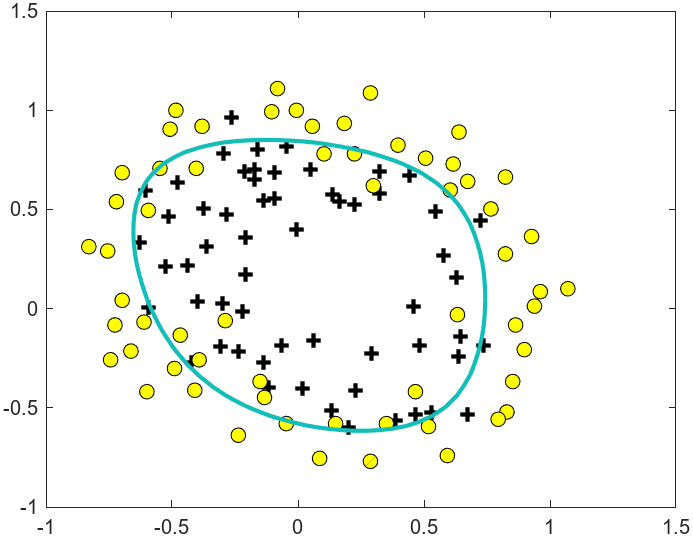
\includegraphics[width=12cm]{regression22} \\ \\
	changes in the dicision boundary as varying \(lambda\) \\ 
	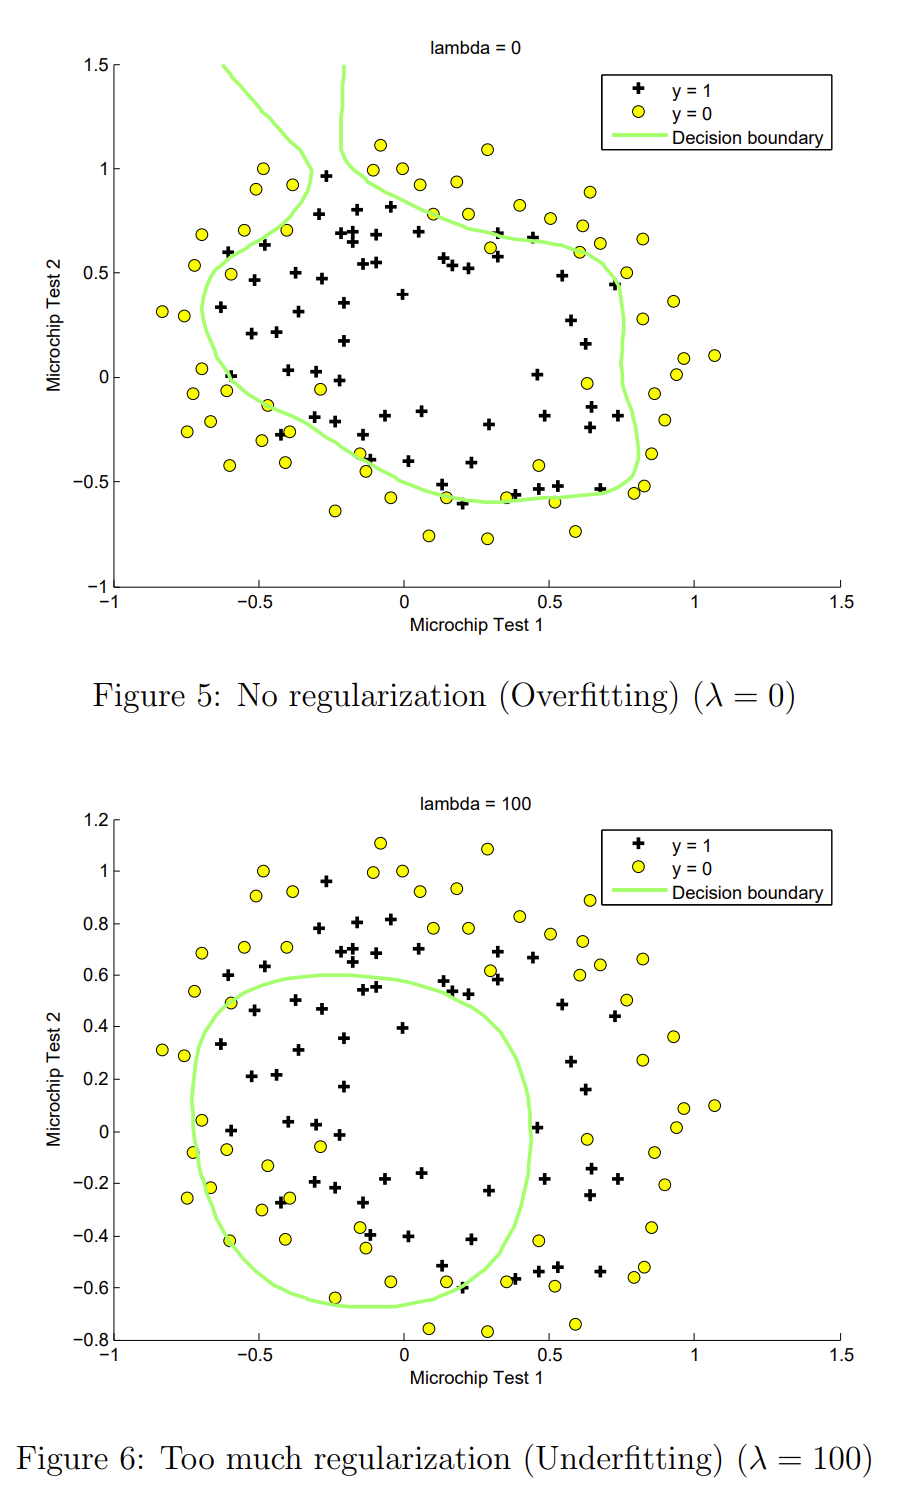
\includegraphics[width=8cm]{lambda}
	
	
	
	
	
	
	
	
	
	
	
	
	
	
	
	
	
	
	
	
	
\end{document}